\section{High-Level Architecture Overview}
\label{sec:architecture_overview}
The prototype developed for this project separates the standard ZK-Rollup pipeline into distinct, containerized microservices. This modular architecture follows Domain-Driven Design (DDD) principles and is explicitly designed to support observability, rapid configuration changes, and controlled benchmarking rather than functioning as a secure production deployment.

The system's end-to-end execution flow is strictly defined as:
\begin{center}
\texttt{Workload Generator $\rightarrow$ Sequencer $\rightarrow$ Executor (gRPC) $\rightarrow$ Submitter $\rightarrow$ L1 Contracts}
\end{center}

This pipeline processes telemetry data by consuming raw JSON/CSV metrics from each component, allowing a Data Tools analytics pipeline to aggregate and analyze the metrics. Local environment execution is orchestrated via \texttt{docker compose} utilizing specific profiles to boot the core stack, the benchmark generator, and the reporting tools. By decoupling the transaction lifecycle—validation, batching, execution/proving, and submission—the prototype enables isolating the specific variables (like batch size or DA mode) required to answer the research questions.

\subsection{Prototype vs. Production Rollup Comparison}
It is critical to distinguish this \textit{research prototype} from a \textit{production rollup}. Production rollups (like zkSync Era or Polygon zkEVM) require full Ethereum Virtual Machine (EVM) compatibility, complex fraud/validity proof mechanisms handling massive state trees, and decentralized sequencer networks designed to prevent censorship. They operate in a Byzantine environment requiring strong liveness and safety guarantees.

In contrast, our prototype operates a \textit{transfer-centric research logic}. It does not implement a full zkEVM. Instead, it implements a simplified state-transition engine tailored for transfer-style workloads and Merkle state updates. Furthermore, the prototype operates in a controlled, non-Byzantine local Hardhat environment. Data Availability (DA) supports calldata and EIP-4844 blobs natively via the L1 node, but off-chain DA is implemented only as a local simulated stub, not a real integration with decentralized networks like IPFS or Celestia. This focused scope allows for precise measurement of specific configuration trade-offs—such as batch size limits or DA selection—without the massive engineering overhead of a production-grade system.

\begin{figure}[H]
    \centering
    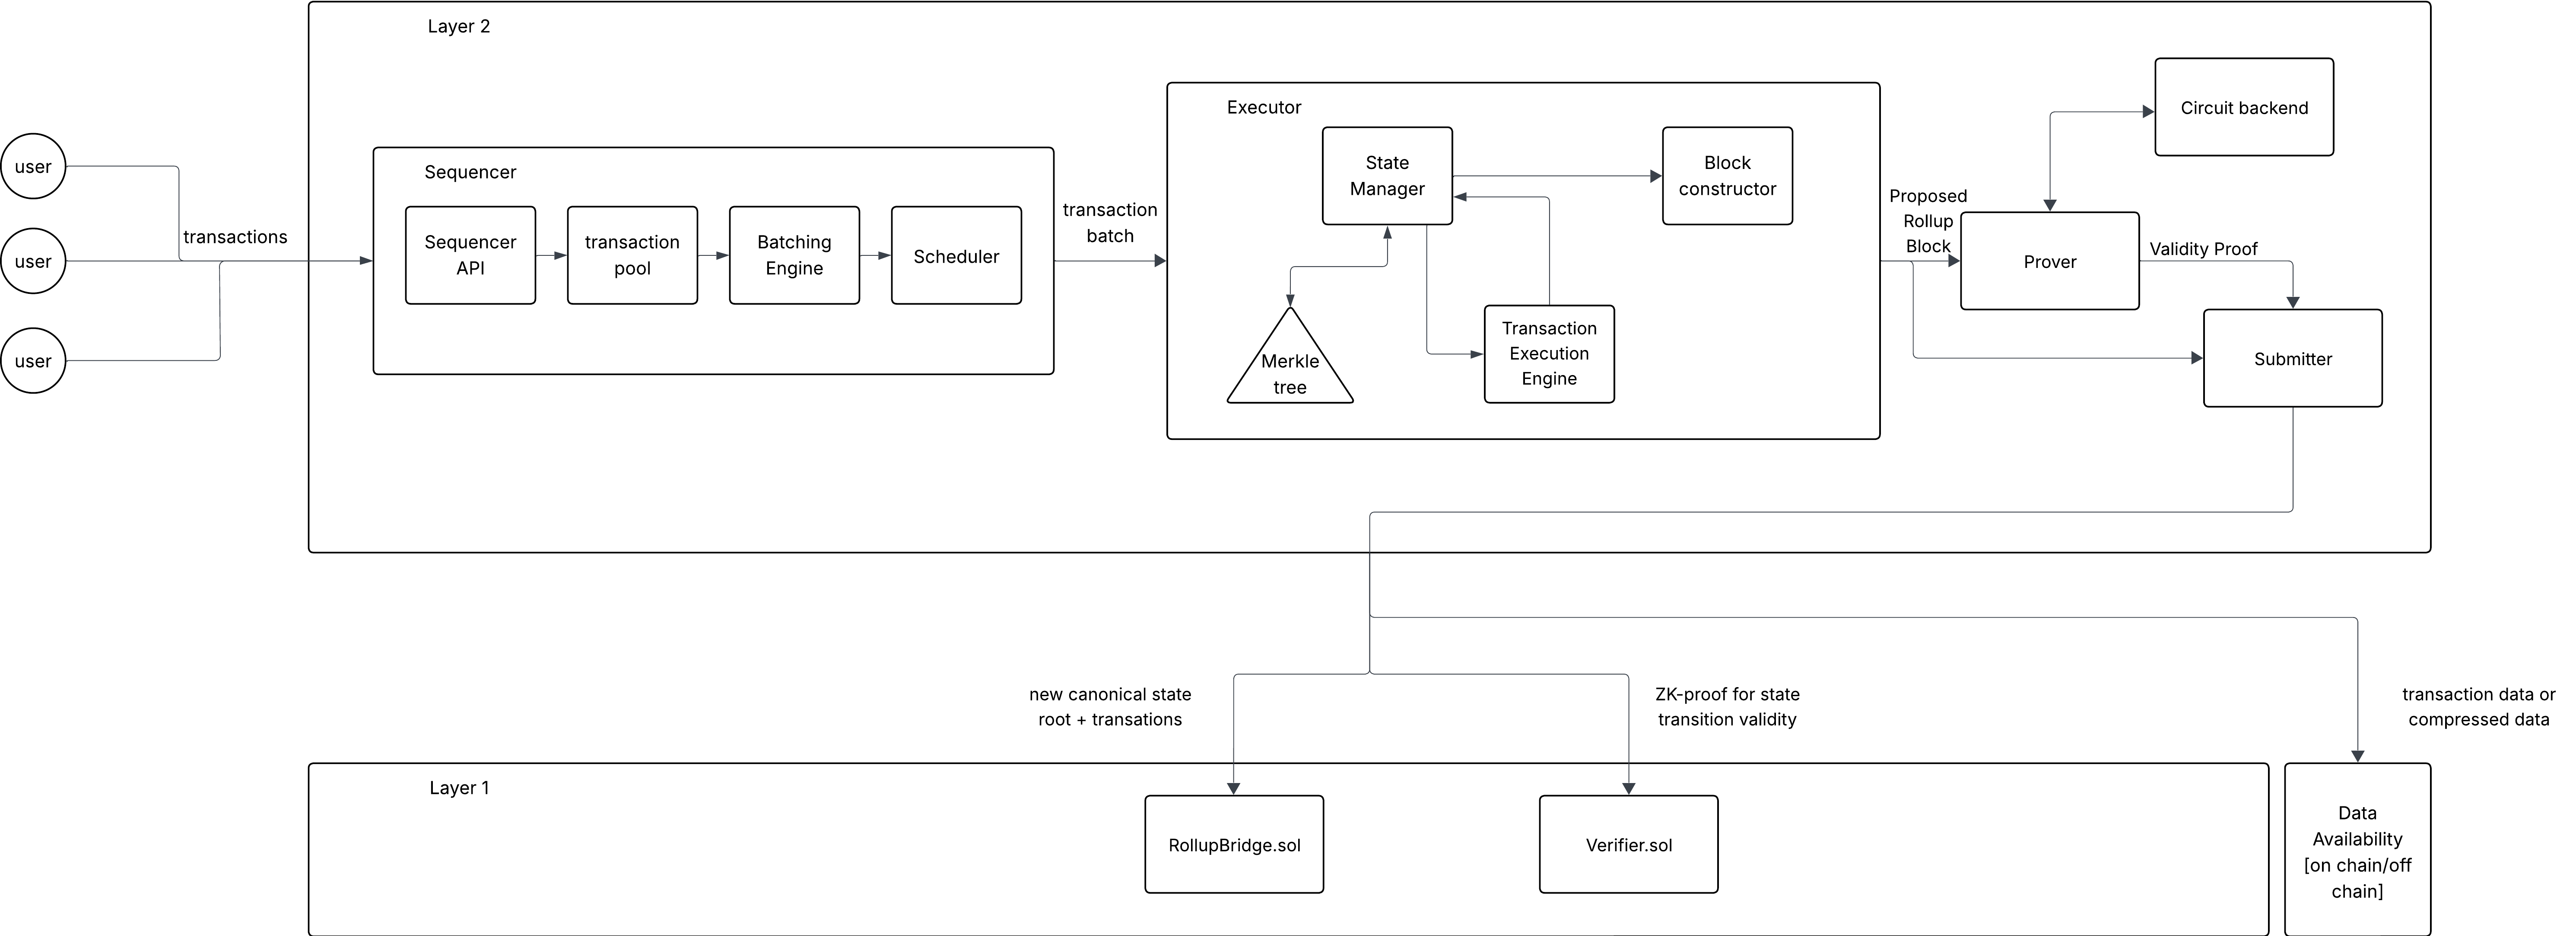
\includegraphics[width=0.90\textwidth]{figures/chapter3/system_architecture.png}
    \caption{High-level architecture of the proposed modular ZK-Rollup benchmarking prototype.}
    \label{fig:system_architecture}

\end{figure}

As shown in Figure~\ref{fig:system_architecture}, the prototype separates transaction ingestion, sequencing, execution, proving, submission, and data availability into modular components.
